\section{Bayesian Decision Theory}
\skriptsubsection{Basics}{20}
\begin{minipage}{9.5cm}
  Let $\omega$ denote the state of nature with possible values $\{\omega_1, \ldots \omega_c\}$.
  $\omega$ is a variable which is described probabilistically.
  The \emph{prior probabilities} are $P(\omega_1) \ldots P(\omega_c)$.
  Possible actions are $\{\alpha_1, \ldots \alpha_a\}$

  For a given measurement $\mathbf{x}$, the \emph{posterior probability} is:
  \begin{center}
    \hilight{$P(\omega_i|x) = \frac{p(x|\omega_i) P(\omega_i)}{p(x)}$} \\
    $= \underbrace{\frac{p(x|\omega_i) P(\omega_i)}{\int\limits_{-\infty}^{\infty}p(x|\omega_j) P(\omega_j) dx}}_{\text{Continous features}}
     \text{ or } 
     \underbrace{\frac{p(x|\omega_i) P(\omega_i)}{\sum\limits_{j=1}^{c}p(x|\omega_j) P(\omega_j)}}_{\text{Discrete features \formelbuch{51}}}$
    \hilight{$ \mathrm{Posterior} = \frac{\mathrm{Likelihood} \; \times \; \mathrm{Prior}}{\mathrm{Evidence}}$}
  \end{center}
  
where we call $p(x|\omega_i)$ the likelihood of $\omega_i$ with respect to $x$,
and $p(x)$ the evidence factor, which is merely a scale factor. \\

The probability of error is the average of all error probabilities:
  \begin{align*}
      P(\error) &= \int_{-\infty}^{\infty} P(\error, x) dx = \int_{-\infty}^{\infty} P(\error|x) p(x) dx \\
  \end{align*}


\skriptsubsection{Continuous Features}{24}
When observing a pattern $\mathbf{x}$ and the true state of nature is $\omega_j$,
the action $\alpha_i$ leads to the \emph{loss} $\lambda(\alpha_i|\omega_j)$.
The conditional risk is then 
$R(\alpha_i|\bfx) = \sum\limits_{j=1}^c \lambda(\alpha_i|\omega_j)P(\omega_j|\mathbf{x})$

The overall risk $R$ must be minimized:
$R = \int R(\alpha(\bfx)|\bfx)p(\bfx) d\bfx$
This is achieved by computing the conditional risk for $i=1,\ldots,a$ 
and selecting the action $\alpha_i$ for which $R(\alpha_i|\bfx)$ is minimal.
The resulting minimum overall risk is called the \emph{Bayes risk} $R^*$.
  
\end{minipage} \vspace{1cm}
\begin{minipage}{9cm}
  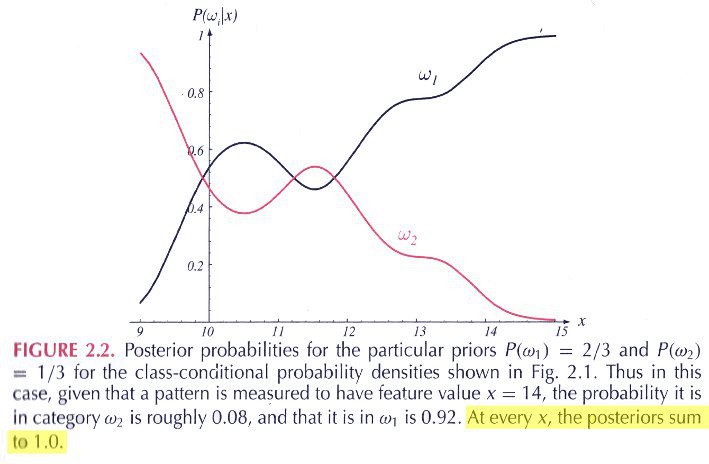
\includegraphics[width=8.5cm]{./images/posterior-prob.jpg}\\
  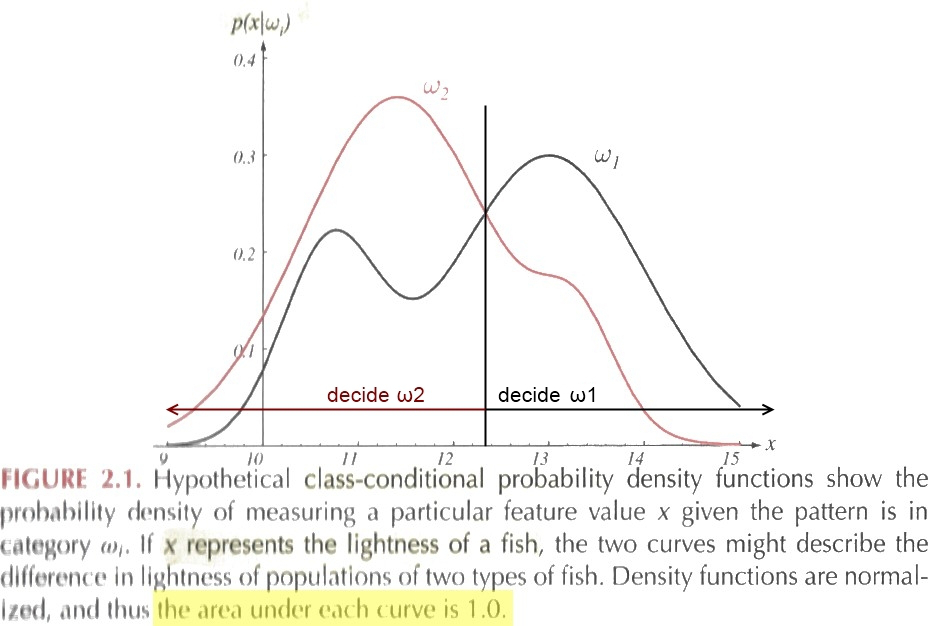
\includegraphics[width=8.5cm]{./images/class-cond-prob.jpg}
\end{minipage}

\skriptsubsection{Two-Category Classification}{25}
Decide $\omega_1$ when
$$\frac{p(\mathbf{x}|\omega_1)}{p(\mathbf{x}|\omega_2)} > \underbrace{
\overbrace{\frac{\lambda_{12} - \lambda_{22}}{\lambda_{21} - \lambda_{11}}}^{\text{=1 for 0-1 assumption}} \frac{P(\omega_2)}{P(\omega_1)}}_{\text{constant}}$$
where $\lambda_{12}$, $\lambda_{21}$ are the costs for a wrong decision and 
$\lambda_{11}$, $\lambda_{22}$ for the correct decision (which are usually $0$).

\skriptsubsection{Classifiers}{29}
\begin{multicols}{2}
    \subsubsection{Multicategory Case}
    Discriminant functions: $g_i(\mathbf{x}) > g_j(\mathbf{x})$ for all $j \neq i$
    $$g_i(\mathbf{x}) = P(\omega_i|x) = 
    \frac{p(x|\omega_i) P(\omega_i)}{\sum\limits_{j=1}^{c}p(x|\omega_j) P(\omega_j)}$$
    
    \subsubsection{Two-Category Case}
    Decide $\omega_1$ when $g(\mathbf{x}) > 0$:
    \begin{align*}
        g(\mathbf{x}) \equiv g_1(\mathbf{x}) - g_2(\mathbf{x})
        &&\text{or}&&
        g(\mathbf{x}) = \ln \frac{p(\mathbf{x}|\omega_1)}{p(\mathbf{x}|\omega_2)} + \ln \frac{P(\omega_1)}{P(\omega_2)} 
    \end{align*}

\end{multicols}

\skriptsubsection{Normal Density}{31}
  The normal density is a model for the case where the feature vectors $\bfx$ 
  for a given class $\omega_i$ are randomly corrupted versions for a prototype vector $\boldsymbol{\mu}_i$.
  
  \skriptsubsubsection{Univariate Density}{32}
  \begin{minipage}{11.5cm}
  $\varphi(x)=p(x)=\frac{1}{\sqrt{2
  \pi}\sigma}\cdot e^{-\frac{(x-\mu)^2}{2\sigma^2}} = N(\mu ; \sigma^2) \qquad \mu=\expected(x)=\int\limits_{-\infty}^{\infty}{x p(x) dx}$\\ 
  $F(x)=\frac{1}{\sqrt{2
  \pi}\sigma}\cdot \int\limits^{x}_{-\infty}{e^{-\frac{(\tilde{x} -\mu)^2}{2\sigma^2}}} \qquad \sigma^2=\expected\left[(x-\mu)^2\right]=\int\limits_{-\infty}^{\infty}{(x-\mu)^2 p(x) dx}$ \\
  % = N(\mu ; \sigma^2),\tilde{x}} $
  
  \textbf{Standard normal distribution}\\
  
  \begin{tabular}{lll}
      Expected value: & $\expected(X)=\mu$ & (=0 for standard normal dist.)\\ 
      Variance: & $\mathrm{var}(X)=\sigma^2$ & (=1 for standard normal dist.)\\
      $x=\dfrac{X-\mu}{\sigma}$ & $x$ aus Tabelle & \\
  \end{tabular} \\
  $ 68\% $ of all values lie within $[ \mu - \sigma, \mu + \sigma]$,
  $ 95\% $ within $[ \mu - 2\sigma, \mu + 2\sigma]$, and 
   $99.7\% $ within $[ \mu - 3\sigma, \mu + 3\sigma]$
  \end{minipage}\hspace{0.5cm}
  \begin{minipage}{7cm}
  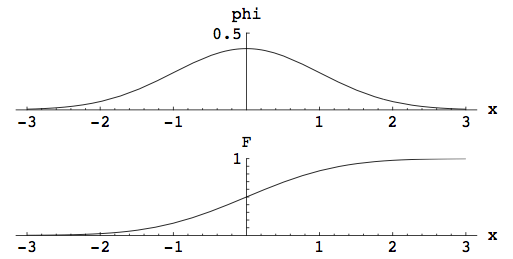
\includegraphics[width=7cm]{images/normalverteilung.png}
  Probability density function and cumulative distribution function of the normal distribution. 
  \end{minipage} \\ \\ 




\skriptsubsubsection{Multivariate Density}{33}
  \begin{equation*}
      N(\boldsymbol{\mu}, \boldsymbol{\Sigma}) \backsim p(\mathbf{x}) = \frac{1}{(2\pi)^{d/2} | \boldsymbol{\Sigma}|^{1/2}} \exp \bigg[-\frac{1}{2} (\mathbf{x} - \boldsymbol{\mu})^T \boldsymbol{\Sigma}^{-1} (\mathbf{x}-\boldsymbol{\mu})\bigg]
  \end{equation*}

  \subsubsubsection{The whitening transform}\formelbuch{34} leads to a proportional matrix of the identity matrix $\mathbf{I}$:
  $\mathbf{A}_w = \boldsymbol{\Phi} \boldsymbol{\Lambda}^{-1/2}$ 
  where $\mathbf{\Phi}$ is matrix whose columns are the orthonormal eigenvectors of 
  $\mathbf{\Sigma}$ and $\mathbf{\Lambda}^{1/2}=\begin{bmatrix}
  \sqrt{\lambda_1}& 0 & \ldots \\
  0&\sqrt{\lambda_2}&\ldots\\
  \ldots
  \end{bmatrix}$ its eigenvalues.
  
  \subsubsubsection{Mahalanobis Distance}\formelbuch{35} from $\mathbf{x}$ to $\boldsymbol{\mu}$: $r^2 = (\mathbf{x}-\boldsymbol{\mu})^T \boldsymbol{\Sigma}^{-1} (\mathbf{x}-\boldsymbol{\mu})$ 
  is with the co-/ variance ``normalized'' distance from the given point to the mean.
  
  
  \subsubsection{Covariance}  
  Covariance: $\sigma_{xy} = c_{xy}= \operatorname{Cov}(X,Y) = E((x-E(X))(y-E(Y))) = E(XY^*)-E(X)E(Y)= \underbrace{0}_{\text{falls X,Y unabhängig}}= \underbrace{r_{xy}}_{\text{falls X,Y mittelwertsfrei}}$
  \\
  Covariance matrix: $\operatorname{Cov}(X) = \mathbf{\Sigma} = 
  \bigl(\operatorname{Cov}(X_i, X_j)\bigr)_{i,j=1,\ldots,n} = \begin{pmatrix} 
\operatorname{Cov}(X_1,X_1) & \cdots & \operatorname{Cov}(X_1,X_n) \\
\vdots & \ddots & \vdots \\
\operatorname{Cov}(X_n,X_1) & \cdots& \operatorname{Cov}(X_n,X_n)\end{pmatrix}$\\


  \skriptsubsubsection{Discriminant Functions for the Gaussian Density}{36}
  \label{sec:bayes_discriminant_function}
  \subsubsubsection{Case 1: $\Sigma_i = \sigma^2 I$\formelbuch{36}}\\
  Same variance in all independent features.
  The linear discriminant function turns to: 
  $$g_i(\mathbf{x}) = \mathbf{w}_i^T \mathbf{x} + w_{i0} \quad \text{with} \quad
  \mathbf{w}_i = \frac{1}{\sigma^2}\boldsymbol{\mu}_i \quad \text{and} \quad 
  w_{i0} = -\frac{1}{2\sigma^2} \boldsymbol{\mu}_i^T \boldsymbol{\mu}_i + \ln(P(\omega_i))$$
  
  The decision surface is a plane: $\mathbf{w}^T(\mathbf{x}-\mathbf{x}_0) = 0$ with $\mathbf{w} = \boldsymbol{\mu}_i - \boldsymbol{\mu}_j$ and 
  $\mathbf{x}_0 = \frac{1}{2}(\boldsymbol{\mu}_i+\boldsymbol{\mu}_j) - \frac{\sigma^2}{||\boldsymbol{\mu}_i-\boldsymbol{\mu}_j||^2} \ln\left(\frac{P(\omega_i)}{P(\omega_j)}\right) (\boldsymbol{\mu}_i-\boldsymbol{\mu}_j)$
  
  
  \subsubsubsection{Case 2: $\Sigma_i = \Sigma$\formelbuch{39}}\\
  Some covariance matrix for all classes.
  The linear discriminant function turns to: 
  $$g_i(\mathbf{x}) = \mathbf{w}_i^T \mathbf{x} + w_{i0} \quad \text{with} \quad
  \mathbf{w}_i = \boldsymbol{\Sigma}^{-1}\boldsymbol{\mu}_i \quad \text{and} \quad
  w_{i0} = -\frac{1}{2} \boldsymbol{\mu}_i^T \boldsymbol{\Sigma}^{-1}\boldsymbol{\mu}_i + \ln(P(\omega_i))$$
  
  The decision surface: $\mathbf{w}^T(\mathbf{x}-\mathbf{x}_0) = 0$ \quad with \\
  $\mathbf{w} = \boldsymbol{\Sigma}^{-1} (\boldsymbol{\mu}_i - \boldsymbol{\mu}_j)$ \quad and \quad 
  $\mathbf{x}_0 = \frac{1}{2}(\boldsymbol{\mu}_i+\boldsymbol{\mu}_j) - \frac{\sigma^2}{(\boldsymbol{\mu}_i-\boldsymbol{\mu}_j)^T \boldsymbol{\Sigma}^{-1} (\boldsymbol{\mu}_i-\boldsymbol{\mu}_j)} \ln\left(\frac{P(\omega_i)}{P(\omega_j)}\right) (\boldsymbol{\mu}_i-\boldsymbol{\mu}_j)$
  
  
  \subsubsubsection{Case 3: $\Sigma_i = $ arbitrary\formelbuch{41}}\\
  General case.
  The discriminant function is now quadratic: 
  $$g_i(\mathbf{x}) = \mathbf{x}^T \mathbf{W}_i^T \mathbf{x} + \mathbf{w}_i^T \mathbf{x} +w_{i0} \quad\text{with}$$
  $$\mathbf{W}_i = -\frac{1}{2} \boldsymbol{\Sigma}^{-1} \quad\text{and}\quad
  \mathbf{w}_i = \boldsymbol{\Sigma}^{-1}\boldsymbol{\mu}_i \quad\text{and}\quad
  w_{i0} = -\frac{1}{2} \boldsymbol{\mu}_i^T\boldsymbol{\Sigma}^{-1}\boldsymbol{\mu}_i - \frac{1}{2}\ln(|\boldsymbol{\Sigma}_i|) + \ln(P(\omega_i))$$
  
  The decision surface cannot be described easily anymore as it may contain holes and nonlinear constructions.
  
  Example: \formelbuch{44}
  

\skriptsubsection{Independent Binary Features}{52}
  Every component $x_i$ of vector $\mathbf{x}$ are either 0 or 1. The class-conditional probability is:\\
  $$P(\mathbf{x}|\omega_1)=\prod\limits_{i=1}^d p_i^{x_i}(1-p_i)^{1-x_i} \qquad ( p_i^{x_i}(1-p_i)^{1-x_i} \Rightarrow\text{ either }p_i\text{ or }1-p_i)$$
  where $p_i = \operatorname{Pr}\left[x_i=1|\omega_1\right]$ and $q_i = \operatorname{Pr}\left[ x_i=1 | \omega_2 \right]$.
  
  
  Discriminant function: $g(\bm x) = \sum\limits_{i=1}^d w_i x_i + w_0$ with 
  $w_i = \ln \frac{p_i(1-q_i)}{q_i(1-p_i)}$ and 
  $w_0 = \sum\limits_{i=1}^d \ln \frac{1-p_i}{1-q_i} + \ln \frac{P(\omega_1)}{P(\omega_2)}$
  
  Example: \formelbuch{53}
